\documentclass[conference]{IEEEtran}
\IEEEoverridecommandlockouts
% The preceding line is only needed to identify funding in the first footnote. If that is unneeded, please comment it out.
\usepackage{cite}
\usepackage{amsmath,amssymb,amsfonts}
\usepackage{algorithmic}
\usepackage{graphicx}
\usepackage{textcomp}
\usepackage{xcolor}

\selectcolormodel{cmyk}

\usepackage{tikz, pgfplots}
\pgfplotsset{compat=1.17}
\usetikzlibrary{calc}
\usetikzlibrary{pgfplots.groupplots}
\usetikzlibrary{plotmarks}

\usepackage{ifthen}
\usepackage{xargs}

\def\BibTeX{{\rm B\kern-.05em{\sc i\kern-.025em b}\kern-.08em
T\kern-.1667em\lower.7ex\hbox{E}\kern-.125emX}}
\begin{document}

    \title{A Comparison of Algorithms Playing EvoMan\\
    {\footnotesize \textsuperscript{*}Note: Sub-titles are not captured in Xplore and
    should not be used}
        \thanks{Identify applicable funding agency here. If none, delete this.}
    }

    \author{\IEEEauthorblockN{1\textsuperscript{st} Given Name Surname}
        \IEEEauthorblockA{\textit{dept. name of organization (of Aff.)} \\
            \textit{name of organization (of Aff.)}\\
            City, Country \\
            email address or ORCID}
        \and
        \IEEEauthorblockN{2\textsuperscript{nd} Given Name Surname}
        \IEEEauthorblockA{\textit{dept. name of organization (of Aff.)} \\
            \textit{name of organization (of Aff.)}\\
            City, Country \\
            email address or ORCID}
        \and
        \IEEEauthorblockN{3\textsuperscript{rd} Given Name Surname}
        \IEEEauthorblockA{\textit{dept. name of organization (of Aff.)} \\
            \textit{name of organization (of Aff.)}\\
            City, Country \\
            email address or ORCID}
    }

    \maketitle

    \begin{abstract}

    \end{abstract}

    \begin{IEEEkeywords}
        game-playing agent, artificial intelligence, EvoMan, genetic algorithm, reinforcement learning,
        q-learning, neuroevolution, particle swarm optimization, proximal policy optimization, ppo
    \end{IEEEkeywords}


    \section{Introduction}\label{sec:introduction}


    \section{Problem Description}\label{sec:problem-description}

    \subsection{Environment}\label{subsec:environment}

    EvoMan~\cite{karinemiras,evoman} is a framework for testing competitive game-playing agents.
    This framework is inspired by Mega Man II~\cite{capcom}, the game created by Capcom.
    In the original game, the player would have to beat $8$ opponents and acquire their weapons
    as they are defeated.
    The additional difficulty of EvoMan comes from the fact the player has to defeat all
    the opponents using only the starting weapon.
    The framework is freely available\footnote{\url{https://github.com/karinemiras/evoman\_framework}}
    and it is currently compatible with Python 3.6 and 3.7.
    There is also an extensive documentation
    available\footnote{\url{https://github.com/karinemiras/evoman\_framework/blob/master/evoman1.0-doc.pdf}}.
    The agent will collect information about the environment through 20 sensors (Fig 1):
    \begin{itemize}
        \item 16 correspond to horizontal and vertical distances to a maximum of 8 different opponent projectiles.
        \item 2 correspond to the horizontal and vertical distance to the enemy.
        \item 2 describe the directions the player and the enemy is facing
    \end{itemize}
    \begin{figure}
        \centering
        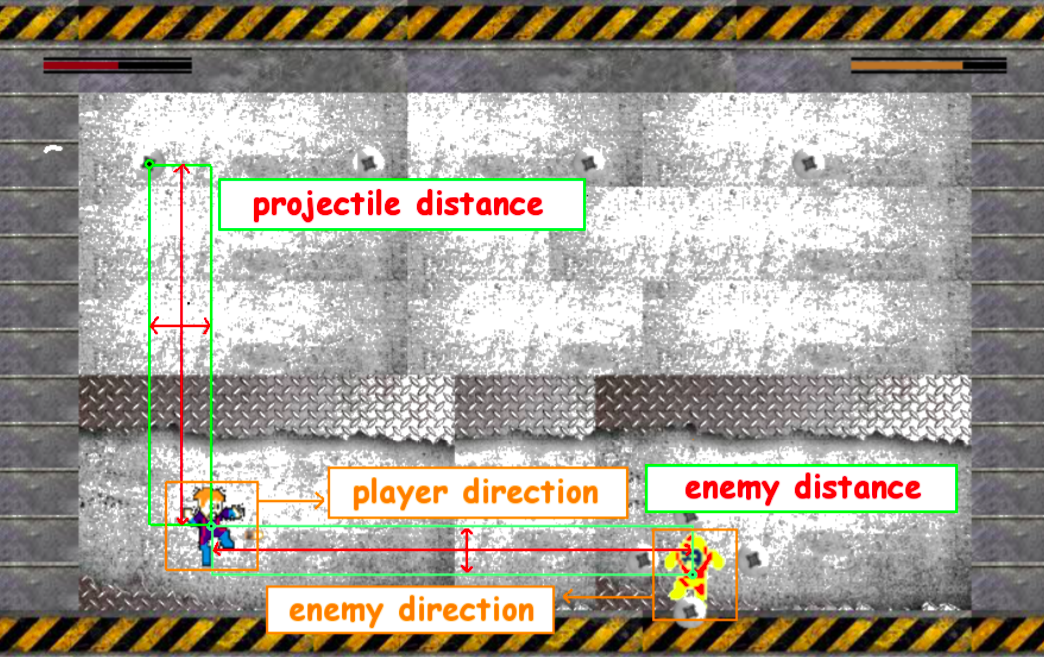
\includegraphics[width=0.5\textwidth]{images/Evoman3.png}
        \caption{Sensors available for the player.}
        \label{fig:sensors}
    \end{figure}
    The actions which the agent may take are:
    \begin{itemize}
        \item walk left
        \item walk right
        \item jump
        \item shoot
        \item release of the jump
    \end{itemize}

    The lives of the player and the enemy start at 100.
    Everytime one of them gets hit, their life deplenishes.
    Whoever's life reaches 0 loses the game.

    \subsection{Problem}\label{subsec:problem}
    The specific problem we are trying to solve is to train an agent on only four of the eight enemies with the purpose
    of maximizing the score gain evaluated against all opponents.
    Since the enemies are very different we should aim for the agent to find generally good strategies like
    aiming towards the opponent and avoiding projectiles.
    The gain of an agent after a game is computed as:
    \begin{gather*}
    gain = 100.01 + player\_energy - enemy\_energy
    \end{gather*}
    The final score metric of an agent is the harmonic mean of the gains against all enemies.

    \subsection{Result Upper Bound}\label{subsec:result-upper-bound}
    (todo: cite https://arxiv.org/pdf/1912.10445.pdf)
    The author of the EvoMan framework trained multiple specialized agents against all opponents.
    The highest final gain, 185.67, was obtained with the NEAT(todo: cite) algorithm.

    \section{Approach}\label{sec:approach}

    \subsection{Q-Learning}\label{subsec:q-learning}

    \subsection{Neuroevolution with Genetic Algorithms}\label{subsec:neuroevolution-with-genetic-algorithms}

    \subsection{Neuroevolution with Particle Swarm Optimization}\label{subsec:neuroevolution-with-particle-swarm-optimization}

    \subsection{Proximal Policy Optimization}\label{subsec:proximal-policy-optimization}

    \subsection{Neuroevolution with Particle Swarm Optimization Bootstrapping and Proximal Policy Optimization}\label{subsec:neuroevolution-with-particle-swarm-optimization-bootstrapping-and-proximal-policy-optimization}


    \section{Experimental Investigation}\label{sec:experimental-investigation}
    cautare 2d - algoritm si puncte de start.
    rezultate partiale si deciziile luate dupa fiecare.


    \section{Results}\label{sec:results}
    informatii despre laptop (pentru ca trebuie mentionat timpul de rulare).
    obs: pentru 1, 6, 7 am obtinut gain mai mare decat orice algoritm specializat (din upper bound)

    \begin{table}[htbp]
        \caption{Table Type Styles}
        \begin{center}
            \begin{tabular}{|c|c|c|c|}
                \hline
                \textbf{Table}&\multicolumn{3}{|c|}{\textbf{Table Column Head}} \\
                \cline{2-4}
                \textbf{Head} & \textbf{\textit{Table column subhead}}& \textbf{\textit{Subhead}}& \textbf{\textit{Subhead}} \\
                \hline
                copy& More table copy$^{\mathrm{a}}$& &  \\
                \hline
                \multicolumn{4}{l}{$^{\mathrm{a}}$Sample of a Table footnote.}
            \end{tabular}
            \label{tab1}
        \end{center}
    \end{table}

    \begin{figure}[htbp]
        \centerline{
\includegraphics{fig1.png}}
        \caption{Example of a figure caption.}
        \label{fig}
    \end{figure}


    \begin{thebibliography}{00}
        \bibitem{b1} G. Eason, B. Noble, and I. N. Sneddon, ``On certain integrals of Lipschitz-Hankel type involving products of Bessel functions,'' Phil. Trans. Roy. Soc. London, vol. A247, pp. 529--551, April 1955.
        \bibitem{b2} J. Clerk Maxwell, A Treatise on Electricity and Magnetism, 3rd ed., vol. 2. Oxford: Clarendon, 1892, pp.68--73.
        \bibitem{b3} I. S. Jacobs and C. P. Bean, ``Fine particles, thin films and exchange anisotropy,'' in Magnetism, vol. III, G. T. Rado and H. Suhl, Eds. New York: Academic, 1963, pp. 271--350.
        \bibitem{b4} K. Elissa, ``Title of paper if known,'' unpublished.
        \bibitem{b5} R. Nicole, ``Title of paper with only first word capitalized,'' J. Name Stand. Abbrev., in press.
        \bibitem{b6} Y. Yorozu, M. Hirano, K. Oka, and Y. Tagawa, ``Electron spectroscopy studies on magneto-optical media and plastic substrate interface,'' IEEE Transl. J. Magn. Japan, vol. 2, pp. 740--741, August 1987 [Digests 9th Annual Conf. Magnetics Japan, p. 301, 1982].
        \bibitem{b7} M. Young, The Technical Writer's Handbook. Mill Valley, CA: University Science, 1989.
    \end{thebibliography}
    \vspace{12pt}
    \color{red}
    IEEE conference templates contain guidance text for composing and formatting conference papers. Please ensure that all template text is removed from your conference paper prior to submission to the conference. Failure to remove the template text from your paper may result in your paper not being published.

\end{document}
